
%(BEGIN_QUESTION)
% Copyright 2007, Tony R. Kuphaldt, released under the Creative Commons Attribution License (v 1.0)
% This means you may do almost anything with this work of mine, so long as you give me proper credit

Suppose you are asked to tune the controller of a liquid flow process.  After obtaining permission from the operator, you analyze the response of the process variable (liquid level) to a 10\% up-and-down step change in the controller output (placed in manual mode):

$$\includegraphics[width=15.5cm]{i01728x01.eps}$$

The first thing you notice is that the PV trend is extremely noisy.  Investigating a little further, you find that the flow transmitter is a differential pressure sensor connected across an orifice plate, and that the transmitter is mounted on a pipe that vibrates a lot.

How does the presence of this noise affect your decisions on how to tune it?  Would you tune this liquid flow controller the same as you would any other liquid flow controller, or would you tune it differently?  Explain your reasoning.

\vskip 20pt \vbox{\hrule \hbox{\strut \vrule{} {\bf Suggestions for Socratic discussion} \vrule} \hrule}

\begin{itemize}
\item{} Identify at least one way this noise could be mitigated, so it no longer posed a challenge to controller tuning.
\item{} Would you recommend re-locating the DP transmitter to a location with less vibration?  Why or why not?
\end{itemize}

\underbar{file i01728}
%(END_QUESTION)





%(BEGIN_ANSWER)

This is definitely a self-regulating process, with negligible dead time.  The fact that it is self-regulating suggests it may be primarily controlled by integral action, and may not need much ``help'' from proportional action at all.  This is good, because proportional action would try to duplicate the PV's noise on the output, to the detriment of the control valve.

Whatever, do {\it not} use any derivative (rate) action on this process!

\vskip 10pt

Follow-up question: does the fact that noise in this process does not influence our tuning decisions much mean that it is okay for this noise to be present?  Why or why not?

%(END_ANSWER)





%(BEGIN_NOTES)

Integral action tends to ignore high-frequency noise, because integration only pays attention to the {\it accumulated error} over time.  Fast up-and-down errors tend to cancel each other out over time.  Another way to think about this is that integration is very similar to first-order lag, which is nothing more than a low-pass filter!

In this case, the noise must be eliminated, but not for the same of control.  Since the source of the noise is mechanical vibration at the measuring instrument (the DP cell), and we know that vibration is ultimately destructive to mechanical devices, we should correct the noise problem for the sake of the transmitter's longevity.

%INDEX% Control, PID tuning: predicting PID requirements based on open-loop response

%(END_NOTES)


